%SOURCE : https://github.com/Gp2mv3/Syntheses
\documentclass[en]{sourcefiles/eplexam} % For a master exam in English, replace fr by en

%\usepackage{sourcefiles/eplcode} % Si l'examen contient du code. La commande pour insérer du code est \begin{lstlisting} ou pour un fichier \lstinputlisting{nomDeFichier}
%\lstset{language={Oz}, morekeywords={for,do,lazy}} % exemple de réglage avec Oz

\graphicspath{{img/}}

\hypertitle{Antennas and propagation}{7}{ELEC}{2910}{2022}{Janvier}{All} % Remplacer Majeure par All si ce n'est pas un cours à option
{Maxime Leurquin}
{Christophe Craeye and Claude Oestges}

%Ce template a pour but de faciliter la rédaction des examens destinés à être posté sur Github. Cependant, il ne peut être posté sans respecter la hiérarchie établie dans le dossier du drive. Il est donc nécessaire de passer par un administrateur du drive (contact.epldrive@gmail.com), ou en suivant les instructions détaillées dans le fichier "How_to_Contribute" sur https://github.com/Gp2mv3/Syntheses. Notez qu'il est possible de contribuer de diverses manières!


%La ligne suivante est à supprimer à la compilation! Cette ligne crée une erreur, mais a été ajoutée afin d'éviter qu'overleaf ne mette du rouge partout.
\begin{document}

\noindent We had 2h to answer everything. There is nothing on the propagation part as it was evaluated only by the project. The exam was open book. We were allowed to use our computers/tablet but not internet of course.

\section{Antenna array}
\noindent An antenna array is located in the XY plane and has $3 \times 3$ elements. Those elements are very short dipoles ( $\sim$ infinitesimal), oriented along X (see figure \ref{enonce}). The phase shift between consecutive elements is $2 \pi / 3$ along $X$ and 0 along $Y$. All elements are excited with the same amplitude. The spacing between elements is $2 \lambda / 3$ along $X$ and $\lambda / 2$ along $Y$, with $\lambda$ being the wavelength.

\begin{enumerate}

    \item Provide a cut of the radiation patterns in the $X Z$ and $Y Z$ planes (5)
    \item What is the direction of maximum of radiation (azimuth and elevation)? (1)
    \item Explain with a drawing why grating lobes have a limited effect, while the spacing between elements is larger than half wavelength (2)
    \item What happens with the grating lobe when the phase shift between elements along $X$ is increased? (1.5)
    \item Propose a simple way to reduce the level of the sidelobes. This can degrade the performance of the array, according to another criterion: which one and why ? (1.5)

\end{enumerate}

\begin{figure}[h]
    \centering
    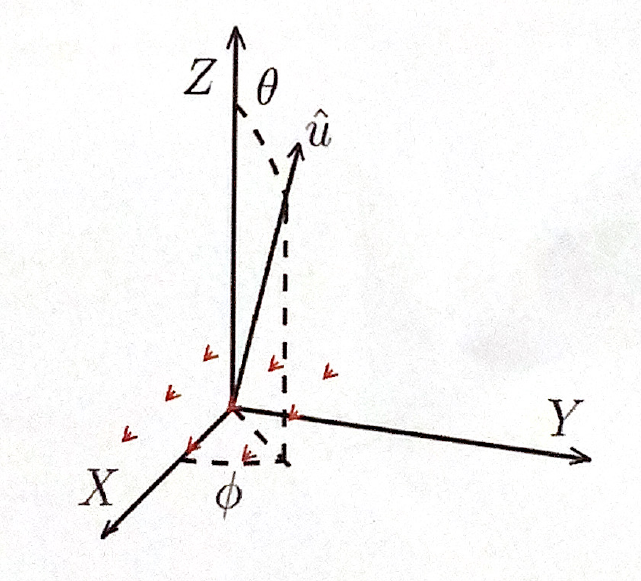
\includegraphics[width=0.5\textwidth]{antennaExamQ1fig.png}
    \caption{}
    \label{enonce}
\end{figure}

\nosolution


\section{}

\noindent A horizontal radio link is established between two antennas, placed on 20 meter high buildings and separated by 100 meters. The central frequency is $10 \mathrm{GHz}$ and the transmitted power is limited to $0.1$ Watt (energy being stored on a supercap). The antennas have a $15 \mathrm{~dB}$ gain. The transmitting antenna radiates circularly polarized waves, while the receiving one produces linear polarization. The noise figure of the receiver is $3 \mathrm{~dB}$ and the bandwidth of the signal is $100 \mathrm{MHz}$. The antenna radiation patterns are symmetrical w.r.t. a horizontal plane passing through the antenna feeding point; the upper half of the pattern sees the cold sky and the lower half sees the warm ground.

\begin{enumerate}
    \item Assuming that the antennas are well matched in terms of impedance, what is the signal-to noise ratio at the output of the receiver ? (5)
    \item Propose dimensions for parabolic reflector antennas in this design (consider $70 \%$ for aperture illumination). (2)
    \item Reflection on the ground can occur. Assuming a reflection coefficient close to $-0.9$, what will be the issue caused by this reflection ? Explain how the radiation pattern can mitigate (a little) the problem and give an approximation for the level of improvement (given that the height of the building is not known exactly, consider a worst-case scenario). (2)
\end{enumerate}

\nosolution

\end{document}


